\documentclass[fleqn,10pt]{wlscirep}
%\documentclass{article}
%\usepackage[margin=1in]{geometry}
\usepackage[utf8]{inputenc}
\usepackage[T1]{fontenc}
\usepackage{xspace}
\usepackage{url}
\usepackage{fancyvrb}
\usepackage{nameref}
\usepackage{hyperref}
\newcommand{\JournalTitle}[1]{#1}

\title{Application Level Cryptography for Securing Online Survey Responses}
\author{Simson L. Garfinkel and William Yates}
%\author[1,*]{Simson L. Garfinkel}
%\affil[1]{US Census Bureau, Suitland, MD}
%\affil[*]{simson.l.garfinkel@census.gov}

%\keywords{Keyword1, Keyword2, Keyword3}

% Abstract goes here for Science abstract
\begin{abstract}
The second Privacy Impact Analysis of the EINSTEIN 3A system developed
by the U.S. Department of Homeland indicated that the system would
have the ability to decrypt the TLS protocol used by the U.S. Census
Bureau to provide confidentiality for responses submitted using
internet self-response tools. To address this potential threat to
confidentiality, the Census Bureau designed an approach using the
World Wide Web Consortium's Web Cryptography API to provide a second
layer of cryptographic protection for respondent data. Two working
prototypes were developed. After further contact with DHS, the
Census Bureau learned that the EINSTEIN 3A's provisions for Web
Content Filtering were designed to decrypt output TLS connections, and
not inbound connections. As a result, the Census Bureau discontinued
development of the prototype. 
\end{abstract}


\newcommand{\ETA}{$\textrm{E}^\textrm{3}\textrm{A}$\xspace}

\begin{document}

%\flushbottom
\maketitle
% Abstract goes here for non-Science abstract
%\begin{abstract}
%\end{abstract}
%\thispagestyle{empty}

\section{Introduction}

The Census Bureau and other U.S. statistical agencies increasingly
rely on Internet-based self-response instruments to collect
data from individuals and establishments. Because Internet-connected
computers have long been under attack by both cyber criminals and
foreign governments\cite{dick-testimony}, these connections are now
subject to monitoring by the U.S. Department of Homeland
Security (DHS).

Respondent data submitted to the Census Bureau website is protected
using the Transport Layer Security (TLS)\cite{rfc8446} cryptographic
protocol and cannot be deciphered by DHS as the DHS monitoring system
is currently deployed.

Because the DHS system might change in the future in response to
new Internet-based threats, the Census Bureau has developed and demonstrated an
approach that uses a second layer of encryption to protect respondent
data. This system would prevent DHS employees from accessing
respondent data even if DHS were to be provided with the Census
Bureau's TLS encryption keys.

\subsection{Background}

The Census Bureau and other U.S. statistical agencies collect
data from respondents under a pledge of confidentiality which states
that data collected will be used for statistical purposes
only. In particular, Title 13 of the U.S. Code prohibits information
that the Census Bureau collects for being used for law enforcement
purposes.

Statistical agencies are increasingly accepting data from respondents
using Internet self-response instruments. In particular, the Census
Bureau plans to make heavy use of Internet self-response for the 2020
Census.\cite{pennington2016} 
At the same time, computers operated by the US Government are under
constant attack. A successful attack on Census Bureau computers would
also represent a significant threat to data confidentiality. For this
reason, the Census Bureau, like other U.S. Government civilian
agencies, participates in the EINSTEIN network monitoring program
operated by the U.S. Department of Homeland Security.\cite{thompson-feb2017}

At the 13th Biennial Federal Committee on Statistical Methodology
(FCSM) Policy Conference, a session explored ``The Challenges of
Overlapping Mandates between Federal Statistical Agencies and
Departmental Chief Information Officers.''\cite{fcsm-program} One of
the panel speakers was Wayne R. Smith, the former Chief Statistician
of Canada and Head of Statistics Canada, who resigned his position in
September 2016 over concerns that the moved to shared information services
meant that Statistics Canada would be unable to
protect the confidentiality of respondent
data\cite{ottawacitizen}. After Dr. Smith spoke, several attendees
expressed concern that the U.S. Government's ``EINSTEIN'' program
might pose a similar threat to confidentiality. 

\subsection{EINSTEIN}

The EINSTEIN program, operated by the U.S. Department of Homeland
Security (DHS), is designed to provide real-time collection,
analysis, and sharing of computer security information across the
federal civilian government to help mitigate this
threat.\cite{dhs-einstein-2004}

The original EINSTEIN program was developed in 2003 and monitored
network flow records between federal civilian executive branch
agencies and the public internet. The goal of this program was to
record data to provide after-action forensic analysis and support. The
EINSTEIN 2 program, first deployed in 2008, incorporated an intrusion
detection system to detect hostile activity against federal agencies
and provide notification to the victims. Four years later, DHS began
transitioning to the EINSTEIN 3 Accelerated (\ETA) program, with the
goal of both detecting and preventing cyber attacks against federal
civilian government networks.\cite{dhs-einstein}

In April 2013, the Department of Homeland Security published 
\emph{Privacy Impact Assessment for EINSTEIN 3 --- Accelerated
  ($E^3A$)}\cite{dhs-e3a-pia}. According to the PIA, ``\ETA combines
existing CS\&C analysis of EINSTEIN 1 and EINSTEIN 2 data as well as
information provided by cyber mission partners with existing
commercial intrusion prevention security services to allow for the
near real-time deep packet inspection of federal network traffic to
identify and react to known or suspected cyber threats.''\cite[p.4]{dhs-e3a-pia}

Designed to be operated by the DHS Office of Cybersecurity and
Communications (CS\&C), EINSTEIN 3's deep packet inspection was
presented as being critical for protecting cyber infrastructure. The
PIA explained that while deep-packet inspection might occasionally
result in the EINSTEIN sensors encountering personally identifiable
information (PII), such information would be immediately deleted if it
was captured (See \nameref{excerpt1}). The PIA also stressed that it
might be necessary, at times, to include PII captured by EINSTEIN in
an analytical product that DHS would then distribute. The PIA further
stated that non-cybersecurity information collected by DHS might be
disseminated for non-cybersecurity purposes (see \nameref{excerpt3}).

On May 6, 2016, DHS issued an update to the \ETA privacy impact
assessment, stating that the system would be enhanced with a new
feature called Web Content Filtering (WCF) that would provide \ETA
with the ability to decrypt the Secure Socket Layer (SSL) protocol
(see \nameref{excerpt4}). (SSL is the
previous name for the Transport Layer Security protocol that is used
to protect World Wide Web traffic)

Consistent with these stated capability improvements in the EINSTEIN
system, on December 14, 2016, the Census Bureau published a Notice in
the Federal Register indicating the intent to revise the
confidentiality pledge.\cite{federal-register-2016-12-14} According to
the announcement, the new pledge would be:

\begin{quote}
  ``The U.S. Census Bureau is required by law to protect your
  information. The Census Bureau is not permitted to publicly release
  your responses in a way that could identify you. Per the Federal
  Cybersecurity Enhancement Act of 2015, your data are protected from
  cybersecurity risks through screening of the systems that transmit
  your data.''\cite{federal-register-2016-12-14,pledge}
\end{quote}

\subsection{Web Content Filtering of Encrypted Content}

Generally speaking, there are two ways that modern web browsers can
communicate with web servers over the Internet: with or without the
use of an encryption protocol called transport layer security
(TLS). When a web page is accessed using a Uniform Resource Locator
(URL) that begins with ``http://'' --- for example,
\url{http://census.gov} --- the connection between the server and the
browser is not encrypted. Alternatively, when the same web page is
accessed using a URL that begins with ``https://''
(e.g. \url{https://census.gov}), then the server and the browser
exchange information over an encrypted channel.  By design, TLS
provides for confidentiality and integrity of the connection: it
assures that a third party cannot eavesdrop on the contents of the
connection, and the data sent by the browser is received by the server
without modification.

TLS is based on public key cryptography. Each web server is configured
with a private key and a public key, which is contained in a public
key certificate. Information encrypted with the private key can only
be decrypted with the public key. When the web browser connects to the
web server, the server sends the browser its public key
certificate. The browser then creates a randomly generated session
key, encrypts the key with the public key and sends it to the
server. The server uses its private key to decrypt the session key so
that the TLS-encrypted communications can take place.

Many commercial network appliances now offer features such as ``Deep
Packet Inspection of SSL/TLS Encrypted
Traffic''\cite{sonicwall}, ``TLS Decryption,''\cite{paloalto} ``SSL
analysis,''\cite{globalsign}. These devices typically operate as a
cryptographic proxy, essentially mounting a man-in-the-middle attack
on the encrypted communications. This is precisely the kind of attack
on confidentiality that TLS was designed to prevent; TLS protections
are bypassed by issuing additional certificates to the TLS inspection
device. A 2016 study by O'Neill et. al found that 1 in 250 TLS
connections on the Internet were proxied. ``The majority of these proxies appear to be benevolent,
however we identify over 1,000 cases where three malware
products are using this technology nefariously,'' the authors concluded.\cite{DBLP:conf/imc/ONeillRSZ16}

Given the widespread availability, use, and apparent acceptance of TLS
decryption technology, we sought to develop a system that would
protect respondent data even if the Census Bureau website was being
monitored with technology that decrypted TLS-protected communications. 
 
\subsection{Securing Respondent Data With the Web Cryptography API}

The World Wide Web Consortium's Web Cryptography API\cite{wcapi}
defines a set of cryptographic functions that can be used by
applications running in modern web browsers. According to the
standard, typical uses for this technology are to enable Multi-factor
Authentication, to encrypt documents locally that are then stored
encrypted on a remote website, to sign documents, and to implement
secure messaging. According to the Can I Use website, the Web
Cryptography API is well supported in all current web browsers except
for Internet Explorer 11 (Figure~\ref{caniuse}).

\begin{figure}
  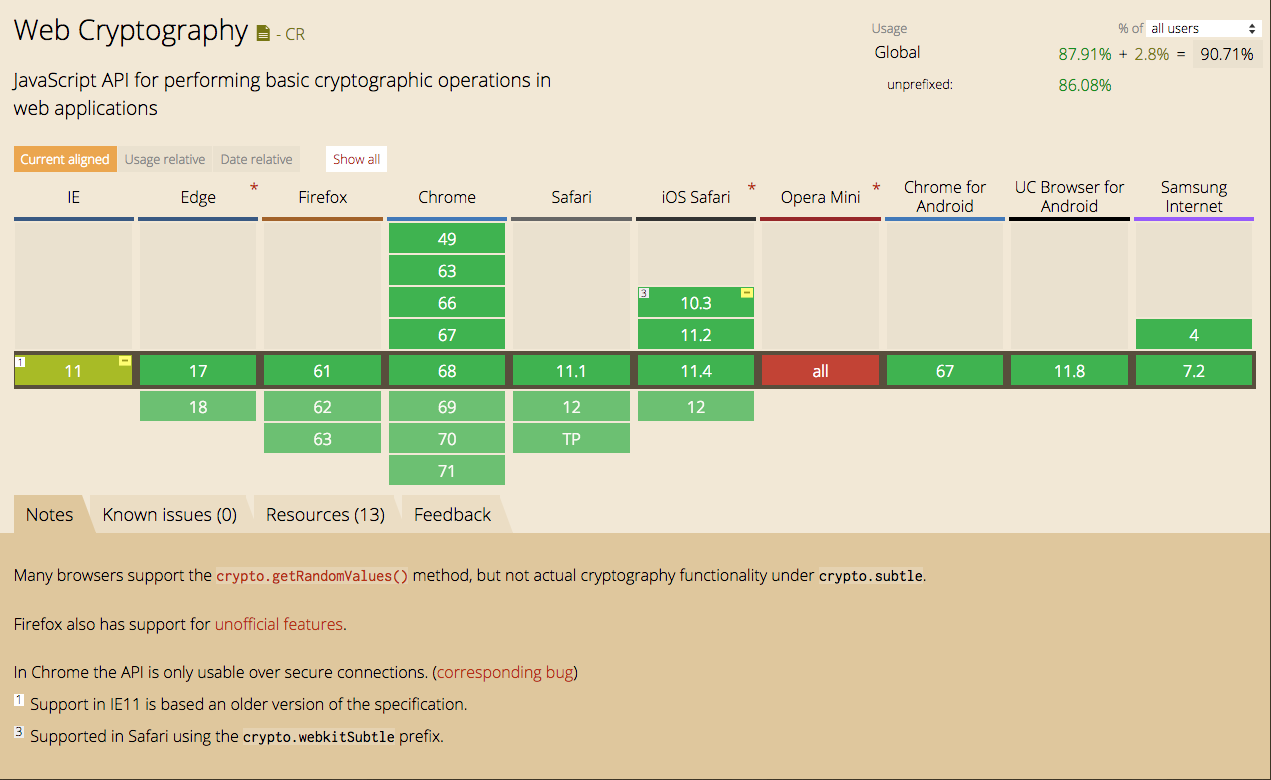
\includegraphics[width=\linewidth]{art/caniuse}
  \caption{Support for the Web Cryptography API as of September 2018,
    according to \url{https://caniuse.com/\#feat=cryptography}.\label{caniuse}}
\end{figure}

The Web Cryptography standard requires that web application using Web
Cryptography API be loaded into a web browser using the TLS protocol, in
order to assure that an attacker does not modify the JavaScript
application as it is being sent to the browser.

The Census Bureau has developed an approach that uses the Web
Cryptography API to encrypt survey responses sent from the
web browser to the web server separately from the underlying HTTPS
technology used to encrypt the web page itself. This second layer of encryption
operates inside the HTTPS encrypted tunnel at the application data
level. It received a second encryption public key and used this second
key to encrypt respondent data, then sent the respondent data to the
web server for decryption. As a result, even if a TLS decryption
appliance was used to decrypt the HTTPS stream, it would not have
access to survey responses.

\subsection{DHS Reactions}

On October 13, 2017, a representative from the Census Bureau met with representatives from the
Department of Homeland Security's National Cybersecurity Protection
System (NCPS) to determine if the application-level encryption system
could be deployed without violating any DHS policy and intentions. At
the meeting, DHS described the operation of the EINSTEIN system and
Census described the application-level encryption approach. DHS stated
that deploying the application-level cryptography system would not violate any
DHS policy. Indeed, DHS stated that it appeared that the system would
provide additional security for Census collected data, by allowing the
data to reside in encrypted form on the Bureau's web server before it
transited to a more secure system.

At the meeting, DHS also stated that in its current deployment, the \ETA Web Content Filtering
was not designed to filter data sent from external web browsers to
Government-operated web servers. Instead, \ETA was solely designed to
monitor data sent between external websites and web browsers operated
within the government networks. For example, \ETA could intercept data
encrypted by malware running inside a user's web browser and
communicating with external web servers.

Following the meeting the October meeting, Census arranged for DHS
NCPS to brief the Federal Committee on Statistical Methodology's
Confidentiality and Data Access subcommittee (on January 23, 2018), as
well as the FCSM executive committee, to explain that \ETA would not
be able to intercept respondent data.

\section{The Application Level Protection Mechanism}

This section describes the application level cryptography mechanism.

\subsection{Overview}

A typical Internet self-response survey consists of three parts:

\begin{enumerate}
  \item A web application server, which sends the HTML survey form to
    the respondent, and receives the respondent data from the
    respondent's web browser.
  \item A Hyper Text Markup Language (HTML) and JavaScript application
    that runs inside the respondent's web browser. This application
    presents the survey to the respondent, receives the data from the user, performs
    local data validation, and sends the data to the application
    server.
  \item A database, which stores the respondent's results. 
\end{enumerate}

Our prototype system modifies these components in the following ways:

\begin{enumerate}
\item The web application server is modified to create a second
  public/private key pair that is used to encrypt respondent data. We
  call this the application-level key pair. In our implementation, the
  server generates a 1024-bit RSA key pair that is used to secure all
  respondent data.
\item Next, we modify the JavaScript application sent from web
  application server to the browser in three ways. First, the
  application-level public key is embedded into the JavaScript
  application. Second, new JavaScript is added that creates a 256-bit
  AES session encryption key to encrypt the respondent data when the user clicks the
  ``SUBMIT'' button. This session encryption key is then encrypted
  with the application-level public key. Finally, the encrypted
  session key and the encrypted respondent data (the ``encrypted
  package'') are sent to the
  application server.
\item We further modify the application server to store the encrypted
  package in the database.
\item Finally, we create a new program for extracting the encrypted
  data from the database and decrypting it. Decryption is performed
  using the application-level private key to decrypt the 256-bit AES
  session key, which is then used to decrypt the respondent data.
\end{enumerate}


\subsection{Demo}

We create a simple web form for a hypothetical survey that requested a
first name and an age (Figure~\ref{survey}). When submitted, these two
values were packed into a JavaScript Object Notation (JSON) data
structure (Figure~\ref{json}), compressed, and encrypted with the session key. The
resulting data (Figure~\ref{encrypted}) was then sent to the web server.

\begin{figure}
  \centering
  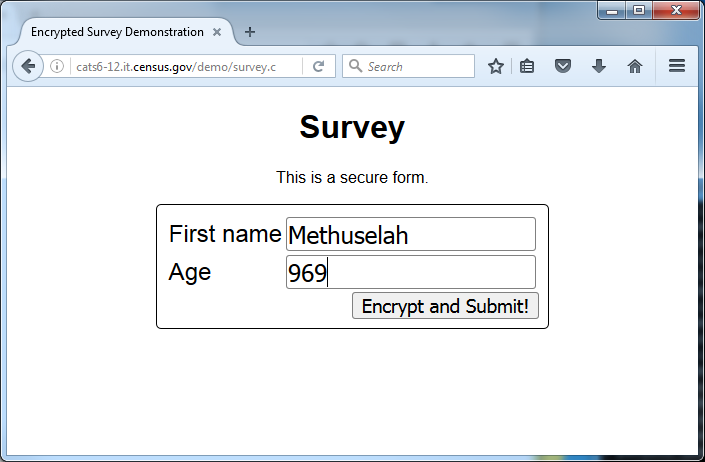
\includegraphics[width=.5\linewidth]{art/figure1}
  \caption{A hypothetical web survey instrument with sample
    data.}\label{survey}
  \end{figure}

\begin{figure}
  \begin{Verbatim}
    {"firstname":"Methuselah","age":"969"}
  \end{Verbatim}
  \caption{A JavaScript Object Notation (JSON) representation of the web response for Figure~\ref{survey}.}\label{json}
\end{figure}

\begin{figure}
  \begin{Verbatim}
    K4lCg6ZlNBi3Wj7jxGuCnPLBAtXVcCDb15yiPlc31bK0bIsXptQ/LC0kU1w4jdop
  \end{Verbatim}
  \caption{An encrypted value.}\label{encrypted}
\end{figure}


\subsection{Prototype}
In our development, we created two distinct prototypes.

The first prototype version encrypted each field of the survey form
using the plain RSA encryption using the PKCS1 v1.5
algorithm. This version of RSA encryption uses the OAEP-based
encryption scheme to protect against chosen plaintext and replay
attacks, but it is not very efficient. 

Our second prototype used the generation of an AES-256 session
key to encrypt the JSON data structure, as described earlier in this
document. In this prototype, the RSA public/private keypair is
separately generated and the public key is explicitly embedded in the JavaScript; in a production
system, the public/private keypair would be stored in appropriately
protected files and dynamically served to the client. The keys are
created with the WebCryptography API and they are only valid for the
duration of the current page, per section 6.2 of the Web Crypto API standard.

Both prototypes implement a client/server system that displays a
simple survey, encrypts the survey results in the user's web browser,
and sends the encrypted results to the web server, where the encrypted
survey responses are stored in a database. A second interface, created
for a demonstration, shows both the encrypted and decrypted values.

The prototype is organized in two directories in the git repository:

\begin{description}
  \item[src/html/demo] Files for configuration and setup of the demo,
    as well as the JavaScript implementation.
  \item[src/cgi-bin/] Software that runs on the web server in response
    to the JavaScript running.
\end{description}

\subsubsection{src/html/demo}
This section describes the contents of the src/html/dmeo directory in
the git repository.

\begin{description}
  \item[config.ini] This configuration file specifies the location of
    the database, the database credentials, and a JSON object that
    specifies the public/private keypair. The key is specified with a
    JSON data object that specifies the parameters $d, e, q, n$ and $p$.
  \item[createdb.sql] The SQL schema for the server database.
  \item[dbutil.py] A python program that can create the database and
    list its contents.
  \item[demo\_random.html] A brief HTML demonstration of generating
    random numbers with JavaScript.
  \item[encrypt.js] JavaScript routines for using the Web Cryptography
    API, used for the first prototype.
  \item[encrypt\_json.js] A revised JavaScript encryption system that
    uses the \verb|window.crypto.subtle.generateKey()| function to
    create an AES-256 key, the \verb|JSON.stringify| method to marshal
    the form values, and the \verb|encrypt_buff| function to encrypt
    the JSON string.
  \item[jquery-3.1.1.min.js] The venerable JQuery JavaScript user
    interface library.
  \item[keyutil.py] A utility program or creating and manipulating
    the RSA keys used in the prototype.
  \item[keyutil\_test.py] Unit tests for the keyutil program.
  \item[notes.txt] Developer notes.
  \item[setup\_rel7.sh] A bash script that installs the necessary
    packages on a Red Hat Enterprise License (RHEL) System 7 Linux
    operating system to run the prototype.
  \item[survey\_json\_report.js] JavaScript for displaying the
      report of successfully encrypted and decrypted survey responses
      for the second prototype.
  \item[survey\_report.js] JavaScript for displaying the
      report of successfully encrypted and decrypted survey responses
      for the first prototype.
\end{description}

\subsection{/src/cgi-bin}
This section describes the contents of the src/cgi-bin directory in
the git repository. This directory contains the Common Gateway
Interface files that are used by the prototype; the files are stored
in a different directory because the RHEL7 secure configuration that
we used required that CGI scripts be stored in a different directory
than the HTML and JavaScript files.

\begin{description}

  \item[report.cgi] A CGI script that displays the secure form and
    shows the public key used to encrypt it.
    \item[submit.cgi] A CGI script that accepts the RSA-encrypted
      form, decrypts the parameters, and stores both the encrypted and
      decrypted values in the database. Note that this script was
      developed for demonstration purposes: in a production system,
      \emph{either} the encrypted or decrypted values would be stored
      in the database, depending on the deployment configuration.
      \item[submit\_json.cgi] A CGI submission script, used by the
        second prototype.
      \item[survey.cgi] A CGI script that displays the survey for the
        first prototype.
      \item[survey\_json.cgi] A CGI script that displays the survey
        for the second prototype.
      \item[survey\_json\_report.cgi] A CGI script that displays a
        report of the submitted values for the second prototype. 
      \item[survey\_report.cgi] A  CGI script that displays a
        report of the submitted values for the first prototype.
\end{description}        


%\bibliographystyle{plainurl}
\bibliography{app-level-crypto}

\section{Conclusion}
We developed a system using the World Wide Web Consortium's Web
Cryptography API that would provide a second layer of cryptographic
protection for survey responses. This second layer was designed to
operate even if some kind of TLS decryption of Web Content Filtering
system was employed between the survey respondent and the internet
self-response instrument.

Although the DHS EINSTEIN 3A system will not be deployed in a way that
will decrypt survey responses, academic research has shown that a
significant portion of internet traffic is now being decrypted using
similar means. Therefore, although it is no longer urgently necessary
to deploy the application level cryptography system described herein,
this or similar technology might be useful in the future to provide an
additional layer of security for survey responses. 

\section{Disclaimer}
This paper is presented with the hope that its content may be of interest to the general statistical community. The views in these papers are those of the authors, and do not necessarily represent those of the Census Bureau.
\section{Additional information}

\subsection{Excerpt from Privacy Impact Assessment for EINSTEIN 3---Accelerated (April 2013)}

\subsubsection{Relationship Between Participants --- Privacy Considerations}\label{excerpt1}
\begin{quote}
  ``CS\&C requires the ability to perform deep packet inspection of known or
suspected cyber threats that are identified by EINSTEIN sensors. CS\&C screens all data
captured by EINSTEIN 1 and EINSTEIN 2 sensors to ensure it is analytically relevant to
a known or suspected cyber threat. \ETA combines existing analysis of EINSTEIN 1 and
EINSTEIN 2 data as well as information provided by cyber mission partners with
existing commercial intrusion prevention security services to allow for the near real-time
deep packet inspection of federal network traffic to identify and react to known or
suspected cyber threats. Network flow records contain only packet header information.
Packet inspection tools allow an analyst to look at the content of the threat data, which
enables a more comprehensive analysis. Packet Capture may contain information that
could be considered PII-like malicious data from or associated with email messages or
attachments. CS\&C follows SOPs regarding handling of information that could be
considered PII including the deletion of any PII unless there is a connection to a known
or suspected cyber threat. Packet Capture shows details about the known or suspected
cyber threat within the federal network. CS\&C analyzes this detailed information and
issues warnings, including possible mitigation strategies to the threat.

  ``In accordance with the SOPs and information handling guidelines, all information
that could be considered PII is reviewed prior to inclusion in any analytical product or
other form of dissemination, and replaced with a generic label when possible. In some
cases, a product may include information that could be considered PII because that
information is deemed analytically relevant and necessary to understand the cyber threat.
In those instances, the SOPs and information handling guidelines provide for safeguards
regarding the marking, dissemination, and handling of the
information.''\cite[p.9]{dhs-e3a-pia}
\end{quote}

\subsection{Privacy Impact Analysis: Related to Information Sharing}\label{excerpt3}
\begin{quote}
  \textbf{``Privacy Risk:} If non-cybersecurity information must be shared outside of DHS, it
increases the risk of unauthorized disclosure.

  \textbf{``Mitigation:} Information about known or suspected cyber threats collected,
analyzed, or otherwise obtained by CS\&C may be disclosed for cybersecurity purposes
and in furtherance of the DHS cybersecurity mission.

Information collected by \ETA or otherwise obtained by CS\&C may be
disseminated for non-cybersecurity purposes in limited situations when the collected
information appears to indicate involvement in activities that may violate laws or
otherwise when the sharing is done in the performance of a lawful government function.
This may include dissemination for law enforcement/intelligence or administrative
purposes unrelated to the protection of an information system from cybersecurity threats,
mitigations against such threats, or response to a cyber incident. In such cases, the
recipient will be a federal, state, or local law enforcement entity.''\cite[p.23]{dhs-e3a-pia}
\end{quote}


\section{Excerpt from Privacy Impact Assessment Update for EINSTEIN 3---Accelerated (May 2013)}
\subsection{Reason for the PIA Update --- Web Content Filtering}\label{excerpt4}
\begin{quote}
``WCF will provide protection for web traffic5
by blocking
access to certain websites that are known to be, or include, malicious content (malware). In
addition, WCF will prevent malware from suspicious websites from running on federal civilian
Executive Branch D/A systems and networks. Finally, WCF will also detect and/or block phishing
attempts as well as the undesirable content that may be included in
those attempts.

``WCF categorizes web-based suspicious traffic, to include all URL/URIs and the content of web sessions,6 which allows system operators to specifically allow or disallow certain types of content that is known to be, or includes, malicious content (malware). WCF service can be configured to alert or block on traffic based on the applicable high-confidence cyber threat indicators and commercial signature development technology (used by the ISP) to allow DHS to block and alert against web-based traffic. This will permit traffic suspected by DHS as malicious as well as customer-specific cybersecurity risk protection requirements to alert or block on specific types of traffic. WCF provides this service via a web proxy between the client and the web server it is attempting to access. The proxy will perform the actions such as redirect, prevent, and/or alert on attempted access to certain (i.e., malicious) web content that matches a DHS cyber threat indicator that may look for a specific URL/URI or webpage content.

``WCF capabilities also include in-line Secure Socket Layer (SSL)
decryption; malware detection; and advanced analytics. WCF SSL
provides visibility into specific types of organizational traffic
(including web content) that has been encrypted, for the purpose of
protecting that traffic from malicious activity that would otherwise
remain hidden by traversing encrypted channels. The capability
decrypts web traffic of D/As participating in the \ETA WCF capability
for the purpose of detecting and preventing malicious web content on
the D/A network.  DHS is not interested in the behavior of
individuals; decryption is focused on web communications, not
communications between individuals. DHS does not use this capability
to investigate the behavior or private content of individuals. Malware
detection is an inherent part of operating WCF. WCF protects specific
federal civilian Executive Branch D/A traffic by using
Government-furnished cyber threat indicators to detect malicious
activity. Advanced analytics in this context refers to behavior-based
(heuristic) threat indicators to identify how a cyber threat or any of
the anomalous characteristics of a cyber threat, a computer system, or
the data behaves.''\cite[pp 2--3]{dhs-e3a-pia2}.
\end{quote}




\end{document}

% LocalWords:  cyber cryptographic cybersecurity mitigations NCPS TLS
%%  LocalWords:  FCSM decrypt decrypted cgi
